\documentclass[main.tex]{subfiles}
\newcommand\numberthis{\addtocounter{equation}{1}\tag{\theequation}}

\newtheorem{theorem}{Theorem}[section]
\newtheorem{definition}{Definition}[section]

\allowdisplaybreaks

\begin{document}
\section{Kernel methods}
Kernel methods is a family of non-parametric techniques. To better explain what it means, we start from what we have already seen in the previous chapters. With parametric method a certain hypothesis in the hypothesis space is defined by the combination of values of the learnable parameters. For example, linear regression is a parametric method, where each hypothesis is defined by the value of the parameters associated with each feature plus the constant term.
With non-parametric methods we have no explicit parameters. %in fact they are somewhat implicit and they depends on the size of the training set. 
In parametric methods the training set is used in the training phase to learn the parameters. Then for the prediction phase the training set is not used because all the relevant information are encoded in the learned model. In non-parametric methods the training set is used also in the prediction phase because the model is implicitly encoded in the dataset.
\paragraph{Example} A very famous example of non-parametric method is the k-nearest neighbour\footnotemark. This method is used for classification. In practice when we have a new sample, we search for the k nearest training data samples in the training data. Then we assign a class to the new sample equal to the most frequent class between the k nearest training samples. Once classified, the new sample becomes part of the training data. \footnotetext{It worth mentioning that k-nearest neighbour is not a kernel method. It's used only as an example for non-parametric methods}

K-nearest neighbour doesn't utilize parameters, but introduce the concept of "distance" for evaluating the new samples. The distance, more formally, is called \textbf{metric}. As in parametric method we need to define the features, in non-parametric methods we need to define a metric. 
We can notice that in the k-nearest neighbour example we have no training time because we haven't a model. But this comes with a price, in fact we have a time penalty during the prediction phase because we need to review each training data to make our assumption, instead of just use our model. 
\begin{itemize}
    \item Parametric: long training time, short prediction time
    \item Non-parametric: short training time, long prediction time
\end{itemize}
So far, all the parametric methods were linear. So in the vanilla configuration they can only solve linear problems. We have also seen how we can extend those linear models to non-linear problems, for both regression and classification through the introduction of the basis functions. In the following sections we will see how we can extend the capability of the linear models to non-linear problems with the \textbf{kernels}.

\subsection{Kernels}
Kernels make linear models work in non-linear settings, by mapping data to higher dimensions, where it may exhibits linear patterns and so linear models are applicable. Another good characteristic of kernel methods is their complexity. In fact, parametric methods complexity is based on the number of features, instead, kernel methods complexity is based on the number of samples. This gives us some advantages in some situation. For example, when we have more features than samples, kernel methods are much more efficient, both complexity and performance wise.
A mapping to higher dimensions can be very expensive to compute, but kernels can give such mapping almost for free. This process is called kernel trick. In practice we can find a dual representation of a linear model using kernels.
\paragraph{Example - Linearize by dimensions augmentation} Consider this binary classification problem

\begin{center}
    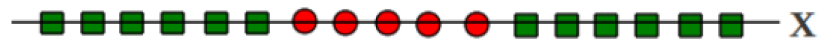
\includegraphics[width=70mm]{img/Add_Dimension.PNG}
\end{center}

Each example is represented by a single feature x. It clearly doesn't exist a linear separator between the two classes. But if we map $\{x\} \rightarrow \{x,x^2\}$ the data are linearly separable.

\begin{center}
    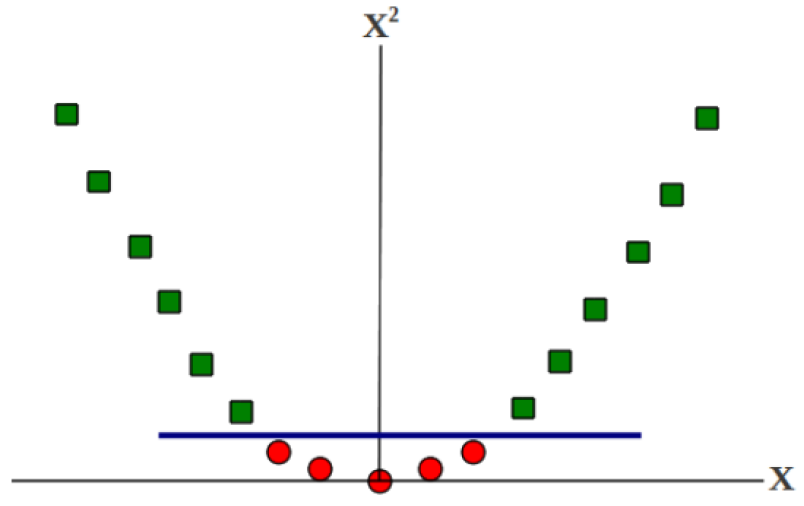
\includegraphics[width=70mm]{img/Add_Dimension2.PNG}
\end{center}
This was the standard approach for extending linear models to non-linear problems

\subsubsection{Kernel functions}
Consider the following mapping $\Phi$ for an example $x=\{x_1, \dots, x_M\}$
\begin{equation*}
    \Phi:x \rightarrow \{x_1^2,x_2^2,\dots,x_M^2,x_1x_2,x_2x_3, \dots,x_1x_M, \dots, x_{M-1}x_M\}
\end{equation*}
This particular mapping is called second order monomial. Each new feature uses a pair of the original features. We can observe that the mapping will increase quadratically the number of features. This will have an impact on complexity because computing the mapping itself can be inefficient. Moreover, using the mapped representation could be inefficient too.
Thankfully, kernels help avoid both these issues because the mapping doesn't have to be explicitly computed and the computations with the mapped features remain efficient.
A kernel is a function which takes as input two data samples, and performs the scalar product between the feature expansions(mapping) of the two samples.
\begin{equation}
    k(x,x') = \Phi(x)^T \Phi(x')
\end{equation}
This kernel function is the metric of our non-parametric method and it measure the similarity between the points $x$ and $x'$. A good consequence of being a scalar product is symmetry($k(x,x') = k(x',x)$)
\paragraph{Example - Linear kernel} Let's consider the simplest kernel possible. The linear kernel correspond to the identity, in fact $\Phi(x) = x$. Given this k(x,x') will be simply the scalar product\footnotemark between the two original samples. The result of the scalar product is maximum when the two vector are pointing in the same direction. \footnotetext{$x \cdot x' = \|x\| \|x'\| \cos{\theta}$, where $\theta$ is the angle between $x$ and $x'$}
\newline
There are different type of kernel
\begin{itemize}
    \item \textbf{Stationary kernel}: Function of difference between arguments. It is called stationary kernel since invariant to translation in space
    \begin{equation*}
        k(x,x') = k(x-x')
    \end{equation*}
    \item \textbf{Homogeneous kernel}: Known as radial basis functions, it depends only on the magnitude of the distance between arguments
    \begin{equation*}
        k(x,x') = k(\|x-x'\|)
    \end{equation*}
\end{itemize}

\subsubsection{Dual representation}
Many linear models for regression and classification can be reformulated in terms of dual representation, in which the kernel function arises naturally. We want this in order to be able to apply the kernel trick. In practice we want to describe our model not using feature but with a kernel. For every linear model exist a dual representation involving kernels. Let's take as an example ridge regression.
We recall that loss function for ridge regression is
\begin{equation*}
    L_w = \frac{1}{2}\sum_{n=1}^N (w^T\Phi(x_n) - t_n)^2 + \frac{\lambda}{2}w^T w
\end{equation*}
and its gradient is
\begin{align*}
    \overset{w}{\nabla}L &= \frac{1}{2} 2 \sum_{n=1}^N (w^T\Phi(x_n) - t_n) \Phi(x_n)^T + \frac{\lambda}{2}2 w^T \\
    &= \sum_{n=1}^N (w^T\Phi(x_n) - t_n) \Phi(x_n)^T + \lambda w^T
\end{align*}
Putting $\overset{w}{\nabla}L = 0$ we have
\begin{align*}
    -\lambda w^T &= \sum_{n=1}^N (w^T\Phi(x_n) - t_n) \Phi(x_n)^T \\
    w^T &= -\frac{1}{\lambda} \sum_{n=1}^N (w^T\Phi(x_n) - t_n) \Phi(x_n)^T \\
    & \text{Define } a_n = -\frac{1}{\lambda} (w^T\Phi(x_n) - t_n) \quad [1x1]\\
    &= \sum_{n=1}^N a_n \Phi(x_n)^T \\
    w &= \bigg( \sum_{n=1}^N a_n \Phi(x_n)^T \bigg)^T \\
    &= \sum_{n=1}^N (a_n \Phi(x_n)^T)^T \\
    &= \sum_{n=1}^N (\Phi(x_n) a_n) \\
    & \text{Define } \Phi = \begin{bmatrix}\begin{bmatrix}\Phi^T(x_1)\end{bmatrix}\\ \vdots \\ \begin{bmatrix} \Phi^T(x_N)\end{bmatrix}\end{bmatrix} \text{, and } a=\begin{bmatrix}a_1 \\ \vdots \\ a_N\end{bmatrix}\\
    &= \Phi^T a \quad [Mx1]
\end{align*}
Now we can substitute w in the loss function. For make the calculus simpler we switch to full matrix notation
\begin{align*}
    L_w &= \frac{1}{2}(\Phi w - t)^T(\Phi w - t)+\frac{\lambda}{2}w^T w \\
    &= \frac{1}{2}(\Phi \Phi^T a - t)^T(\Phi \Phi^T a - t)+\frac{\lambda}{2}(\Phi^T a)^T \Phi^T a \\
    &= \frac{1}{2}(\Phi \Phi^T a - t)^T(\Phi \Phi^T a - t)+\frac{\lambda}{2} a^T \Phi \Phi^T a \\
    &= \frac{1}{2}((\Phi \Phi^T a)^T - t^T)(\Phi \Phi^T a - t)+\frac{\lambda}{2} a^T \Phi \Phi^T a \\
    &= \frac{1}{2}(a^T \Phi \Phi^T - t^T)(\Phi \Phi^T a - t)+\frac{\lambda}{2} a^T \Phi \Phi^T a \\
    &= \frac{1}{2}(a^T \Phi \Phi^T \Phi \Phi^T a) + \frac{1}{2}t^T t -\frac{1}{2} a^T \Phi \Phi^T t -\frac{1}{2} t^T \Phi \Phi^T a +\frac{\lambda}{2} a^T \Phi \Phi^T a \\
    &= \frac{1}{2}(a^T \Phi \Phi^T \Phi \Phi^T a) + \frac{1}{2}t^T t - a^T \Phi \Phi^T t +\frac{\lambda}{2} a^T \Phi \Phi^T a
\end{align*}
We can observe how $\Phi$ is present only when multiplied by its transpose. In this way we can use the kernels we have define before to substitute the features. In order to have a simpler notation, we can observe that the kernel function is a Gram matrix\footnotemark $K=\Phi\Phi^T$ [NxN], where each element is 
\begin{equation*}
    K_{nm} = \Phi(x_n)^T \Phi(x_m) = k(x_n,x_m)
\end{equation*}
\begin{equation}
    K =
    \begin{bmatrix}
    k(x_1,x_1) & \dots & k(x_1,x_N) \\ 
    \vdots & \ddots & \vdots \\
    k(x_N,x_1) & \dots & k(x_N,x_N)
    \end{bmatrix}
\end{equation}
\footnotetext{Given N vectors, the Gram Matrix is the matrix of all inner products. A matrix by its transpose is always a Gram matrix}

\paragraph{Notes} 
\begin{itemize}
    \item $\Phi$ [NxM] and $K$ [NxN]
    \item K is a matrix of similarities of pairs of samples(metric)
    \item K is symmetric
\end{itemize}
Now we can substitute $\Phi^T \Phi$ with $K$. We write $L_w$ as $L_a$ because w is no longer present in the equation so $L_a$
\begin{equation*}
    L_a = \frac{1}{2}(a^T K K a) + \frac{1}{2}t^T t - a^T K t +\frac{\lambda}{2} a^T K a
\end{equation*}
Solving for $a$ by combining $w=\Phi^T a$ and $a_n=-\frac{1}{\lambda}(w^T \Phi(x_n)-t_n)$
\begin{equation}
    a = (K + \lambda I_N)^{-1} t \quad [Nx1]
\end{equation} \label{eqn_a}
Solution for $a$ can be expressed as a linear combination of elements of $\Phi$, whose coefficients are entirely in terms of kernel $k(x,x')$, from
which we can recover original formulation in terms of parameters $w$. This means that the loss function is convex thus it has only one global minimum. We can observe how all the element in equation (\ref{eqn_a}) have dimension dependent only on the number of samples. This is exactly what we were looking for, because we have said that the complexity of kernel methods depends on the number of samples and not features. It practically means that now we have to invert a [NxN] matrix instead of a [MxM].

When we make a prediction for a new x we have our linear regression model. If we substitute $w=\Phi^Ta$.
\begin{align*}
    y(x) &= w^T\Phi(x) \\
    &= a^T\Phi \Phi(x) \\
    &\text{Define }k(x)=
    \begin{bmatrix}
    k(x,x_1) \\
    \vdots \\
    k(x,x_N)
    \end{bmatrix} \\
    &= k(x)^T (K + \lambda I_N)^{-1} t
\end{align*}
As we can see, the prediction is a linear combination of the target values from the training set. We can get a very nice intuition of this. Making a linear combination of the target values is like taking a weighted average over the target samples, based on the similarity between the new samples and the target samples in the training data. In this way, we have completely eliminated the parameters, so we have found a dual representation of the parametric model eliminating the need of parameters and features, for describing the model, by using kernels. So the "model" is now implicit in the data.
This approach have several advantages
\begin{itemize}
    \item Solution for a is entirely described in terms of kernel s functions. Once we get $a$ we can recover $w$ as a linear combination of $\Phi$ using $w = \Phi^T a$
    \item When computing the solution we need to invert a [NxN] matrix and not a [MxM] matrix. This is good when the number of features is very high
    \item The true advantage is that for some kernel, we don't even need to compute $\Phi$. Doing so we resolve a lot of issues revolving around the high number of features. We will see how we can work even with infinite features.
    \item Kernel functions can be defined not only over simply vectors of real numbers, but also over objects as diverse as graphs, sets, string, and text documents
\end{itemize}

\subsubsection{Kernel construction}
In this section we will see how we can construct a kernel. If you are wondering how the heck we can avoid to compute $\Phi$ directly, even if $K=\Phi^T \Phi$, you are in the right section.
So the most naive way to construct a kernel is through the scalar product of $\Phi$ by its transpose. Nothing special, in fact we don't have any special gain doing this because we still need to use $\Phi$.
\begin{equation*}
    k(x,x') = \Phi(x)^T \Phi(x') = \sum_{i=1}^M \Phi_i(x) \Phi_i(x')
\end{equation*}
Where $\Phi(x)$ are basis functions.

It exist a second and much more interesting method to construct kernels. We choose a function that correspond to a scalar product in some space. We make an example to better understand what it means.
\paragraph{Example}Suppose to have the kernel function $k(x, z) = (x^T z)^2$.
To be a valid kernel we need to find a features expansion that is able to provide the same result as the initial kernel definition. Suppose we are in two dimensional space.
\begin{align*}
    k(x,z) &= (x^T z)^2 \\
    &= (x_1z_1 + x_2z_2)^2 \\
    &= x_1^2z_1^2 + 2x_1z_1x_2z_2 + x_2^2z_2^2 \\
    &= \begin{bmatrix} x_1^2 & \sqrt{2}x_1x_2 & x_2^2\end{bmatrix}\begin{bmatrix} z_1^2 & \sqrt{2}z_1z_2 & z_2^2\end{bmatrix}^T \\
    &= \Phi(x)^T \Phi(z)
\end{align*}
So what's the point? We have checked if $k(x,z)$ is a valid kernel by finding a feature expansion whose inner product is equal to the kernel. Furthermore we can notice that the feature mapping takes the form $\begin{bmatrix} x_1^2 & \sqrt{2}x_1x_2 & x_2^2\end{bmatrix}$, comprising all second order terms with a specific weighting. The very nice thing about this is that we can avoid to compute $\Phi$ and then perform the scalar product, because we can directly estimate the kernel function(metric). Computing directly the kernel is way cheaper than computing $\Phi$.
In this case we have
\begin{itemize}
    \item \textbf{Naive kernel construction}: compute 6 features values and 9 multiplication for inner product
    \item \textbf{Direct estimation of valid kernel}: 2 multiplication and a squaring
\end{itemize}
This is a very simple example and the gain is very small. If we consider the kernel $k(x,z) = (x^T z + c)^p$, we can demonstrate that the feature expansion that represent this kernel includes all the possible monomial from degree 0 to p.
\begin{itemize}
    \item \textbf{Naive kernel construction}: exponential grow in number of operation
    \item \textbf{Direct estimation of valid kernel}: linear grow in number of operation
\end{itemize}
We can represent features expansion that include billions of elements with very simple kernel which need few operation to be computed.
in this way we have construct a memory based method which doesn't use both features and weights, but it exploit the training data to predict new samples.

Now we can define more formally how we can demonstrate that a given kernel is valid.
Necessary and sufficient condition for a function $k(x, x')$ to be a kernel is that the gram matrix $K$, whose elements are given by $k(x_n, x_m)$, is positive semi-definite\footnotemark for all possible choices of the set $\{x_n\}$.
\footnotetext{Positive semi-definite means that $x^T K x \geq 0,$ $\forall x:x_i\in \mathbb{R}^+$. A notable consequence is that a positive semi-definite matrix has}
\begin{theorem}[Mercer’s theorem]
Any continuous, symmetric, positive semi-definite kernel function $k(x, y)$ can be expressed as a dot product in a high-dimensional space
\end{theorem}
New kernels can be constructed from simpler kernels as building blocks.
Be aware that a really meaningful kernel is the one that define a good metric for representing the similarity between two inputs. 
So given kernels $k_1(x,x')$ and $k_2(x,x')$, the following new kernels will be
valid
\begin{enumerate}
    \item $k(x,x') = ck_1(x,x')$
    \item $k(x,x') = f(x)k_1(x,x')f(x')$, where $f(\cdot)$ is any function
    \item $k(x,x') = q(k_1(x,x'))$, where $q(\cdot)$ is a polynomial with non-negative coefficients
    \item $k(x,x') = exp(k_1(x,x'))$
    \item $k(x,x')$ = $k_1(x,x')+k_2(x,x')$
    \item $k(x,x')=k_1(x,x')k_2(x,x')$
    \item $k(x,x')=k(\Phi(x),\Phi(x'))$, where $\Phi(x)$ is a function from x to $\mathbb{R}^M$
    \item $k(x,x') = x^TAx'$, where $A$ is a positive semi-definite matrix
    \item $k(x,x') = k_a(x_a,x_a') + k_b(x_b,x_b')$, where $x_a$ and $x_b$ are variables with $x=(x_a,x_b)$
    \item $k(x,x')=k_a(x_a,x_a') k_b(x_b,x_b')$
\end{enumerate}
\paragraph{Example - Gaussian kernel} A commonly used homogeneous kernel is the Gaussian kernel.
\begin{equation}
    k(x,x') = exp \bigg(-\frac{\|x-x'\|^2}{2\sigma^2} \bigg)
\end{equation}
Being an homogeneous kernel, it's based on a distance metric. In particular $\|x-x'\|^2$ represent the euclidean distance between $x$ and $x'$.
\begin{proof}[Gaussian kernel validity]
We can demonstrate its validity through kernel composition.
We can expand the square as
\begin{equation*}
    \|x-x'\|^2 = x^Tx + x'^Tx' -2x^Tx'
\end{equation*}
To give
\begin{align*}
    k(x,x') &= exp(-\frac{1}{2\sigma^2} k_1(x,x')), \quad \text{where} \\
    k_1(x,x') &= x^Tx + x'^Tx' - 2x^Tx'
\end{align*}
We know that the exponential of a valid kernel is still valid(4) so we need to demonstrate that $-\frac{1}{2\sigma^2}k_1(x,x')$ is valid.
For composition (1) we need to demonstrate that $k_1(x,x')$ is valid because $\frac{1}{2\sigma^2}$ is only a coefficient. We also know that for (5) the sum of valid kernel is still valid, so we need to verify the components of $k_1(x,x')$. All three components are just linear kernels with some coefficient(1), so they are valid.
\end{proof}
Here we can appreciate the power of kernel composition. In fact, we don't know which is the feature expansion of the Gaussian kernel, but we are sure that it exists. This is once more a demonstration of how kernel methods don't need to define the features. Still, they correspond to the dual representation of a parametric model, where, in the case of Gaussian kernel, the number of features is infinite.

We can also expand the Gaussian kernel to non-Euclidean distances
\begin{equation}
    k(x,x') = exp\bigg( -\frac{1}{2\sigma^2}(k_i(x,x) + k_i(x',x') - 2k_i(x,x'))  \bigg)
\end{equation}

\paragraph{Object kernels}
We have said how kernels can be defined over real vector numbers but also object such as sets, graph, strings and text.
\paragraph{Example - Sets} To define a simple metric over sets we can use
\begin{equation}
    k(A_1,A_2) = 2^{|A_1 \cap  A_2|}
\end{equation}
In practice, we find the number elements included in both $A_1$ and $A_2$. Then we use this number as an exponent.
\paragraph{Example - Generative models} We define the generative model $p(x)$ which is a mapping in a one-dimensional feature space. The kernel is defined as
\begin{equation}
    k(x,x') = p(x)p(x')
\end{equation}
p(x) represent a probability. Performing the multiplication between $p(x)$ and $p(x')$ is like doing a inner product in a one-dimensional space so the kernel is valid. In practice we are multiplying the probability of $x$ and $x'$. So the kernel defines the probability of having both $x$ and $x'$ and so their "similarity".

\subsection{Gaussian processes}
In the previous sections, we have seen how we can find the dual representation of ridge regression based on kernels. Gaussian processes are the kernel version of the Bayesian linear regression when we assume a Gaussian distribution for both prior and likelihood. So far, we have seen how to find the dual model of a non-probabilistic model for regression like ridge regression. We can extend the dual formulation to probabilistic discriminative models.

In Bayesian linear regression we have introduced a prior distribution over the parameters. Given a training set, we evaluate a new distribution over the parameters(posterior) by combining the prior and the new data observed(likelihood). From the posterior we can find a predictive distribution $p(t|x)$ for a new input x. With Gaussian processes, we define directly a prior distribution over functions\footnotemark. \footnotetext{With function we indicate the model in the parametric world. So in linear regression it would be the hyperplane defined by the parameters}
If before we defined a prior over the parameters associated to the function, now we define a prior directly on the functions, bypassing the parameters.
If we recall that Gaussian processes are actually kernel method we can make sense of it.
With parametric method the function(model) is defined by its parameters, which decide the "shape" and characteristics of the function.
In non-parametric method, the function is defined by the samples. Now we can observe that to define a function with samples, we would need a infinite amount of them. So what Gaussian processes are doing is considering an infinite collection of variables, one for each input point, and considering them as jointly distributed as a infinite-dimensional Gaussian distribution. OK, don't panic now we will see some graph and it will be clearer.
\paragraph{Example - Gaussian processes intuition}
We plot a function. To define the function we should consider infinite points. For this example we only consider two points $x_1$ and $x_2$. For each point we define $p(t|x)$ as a Gaussian distribution. Then, we join the two points distribution in a multivariate Gaussian. 
This distribution describe the values of our function based on the inputs x. Note that the variables are not independent, because the value of consequent inputs are likely to have similar values.
\newpage
\begin{center}
\begin{tabular}{cc}
    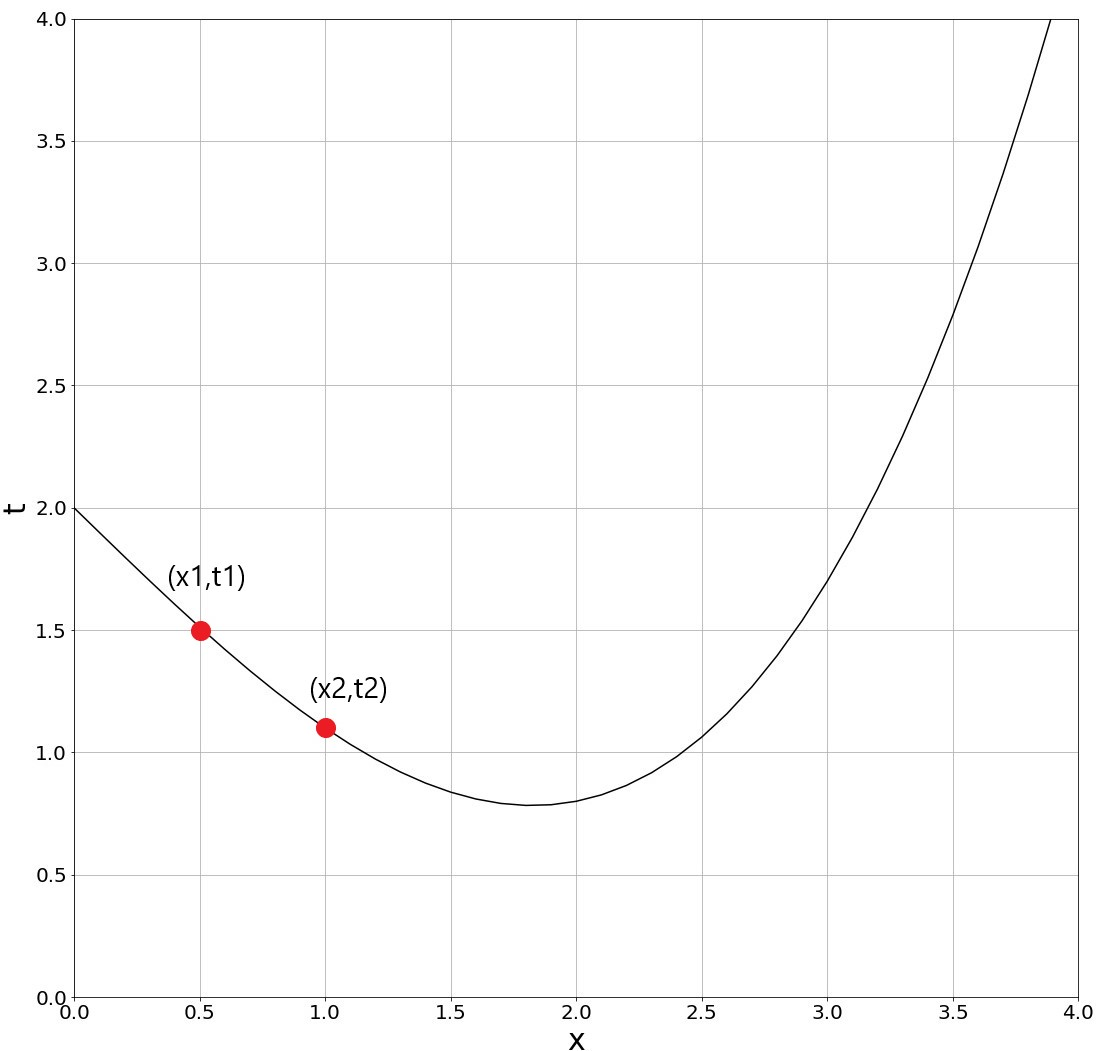
\includegraphics[width=80mm]{img/GaussianProcesses.jpg} &
    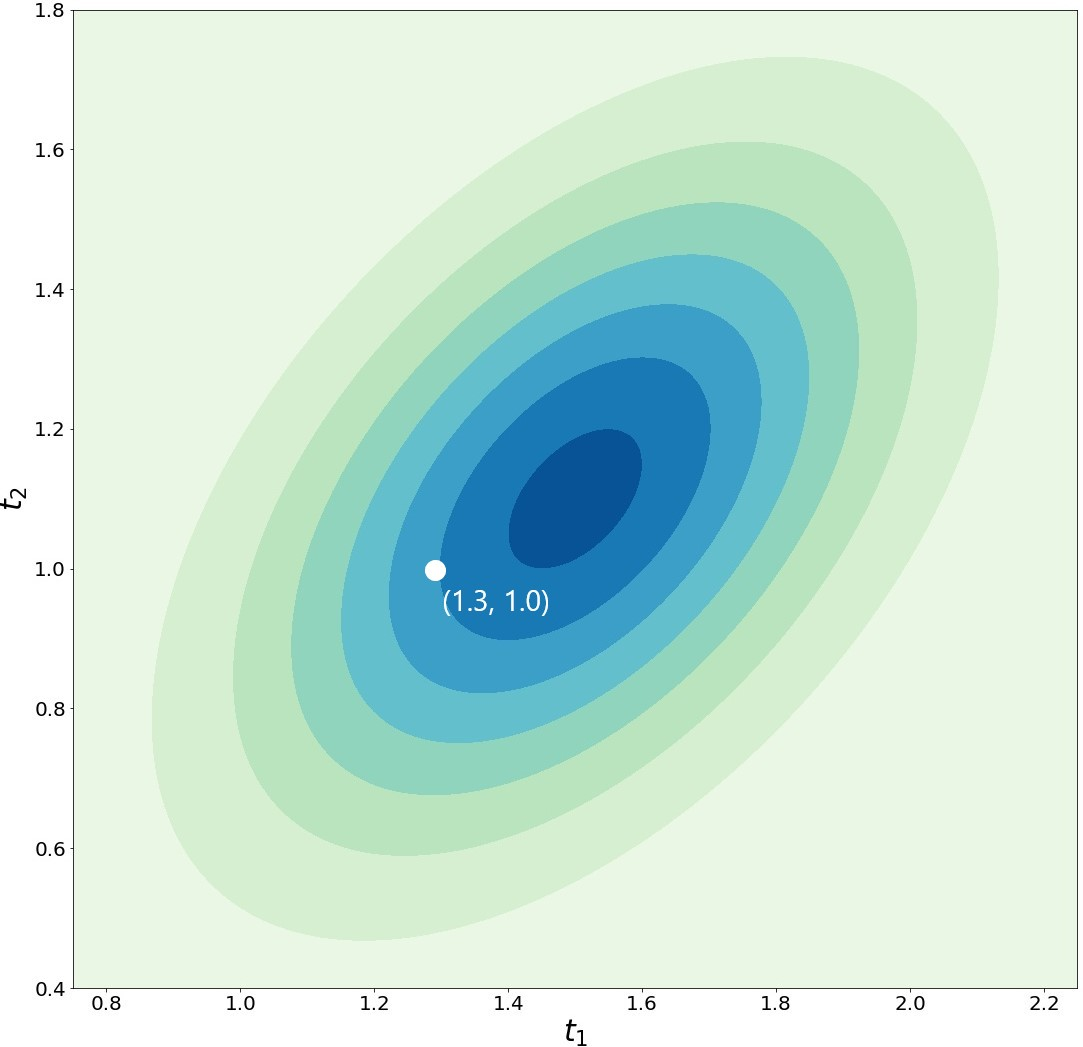
\includegraphics[width=80mm]{img/MultivariateGaussian.jpg} \\
(a) Function we want to estimate & (b) Multivariate Gaussian over t
\end{tabular}
\end{center}
If we draw a sample from the multivariate Gaussian we would define a new function. In fact, picking a sample is the same as picking an infinite sequence of points in the $(x,t)$ system. So our goal is to define a multivariate Gaussian which describe as well as possible the values of every point of our original function. The white dot in figure (b) is a sample of the multivariate Gaussian representing a guess on the original function.
\begin{center}
    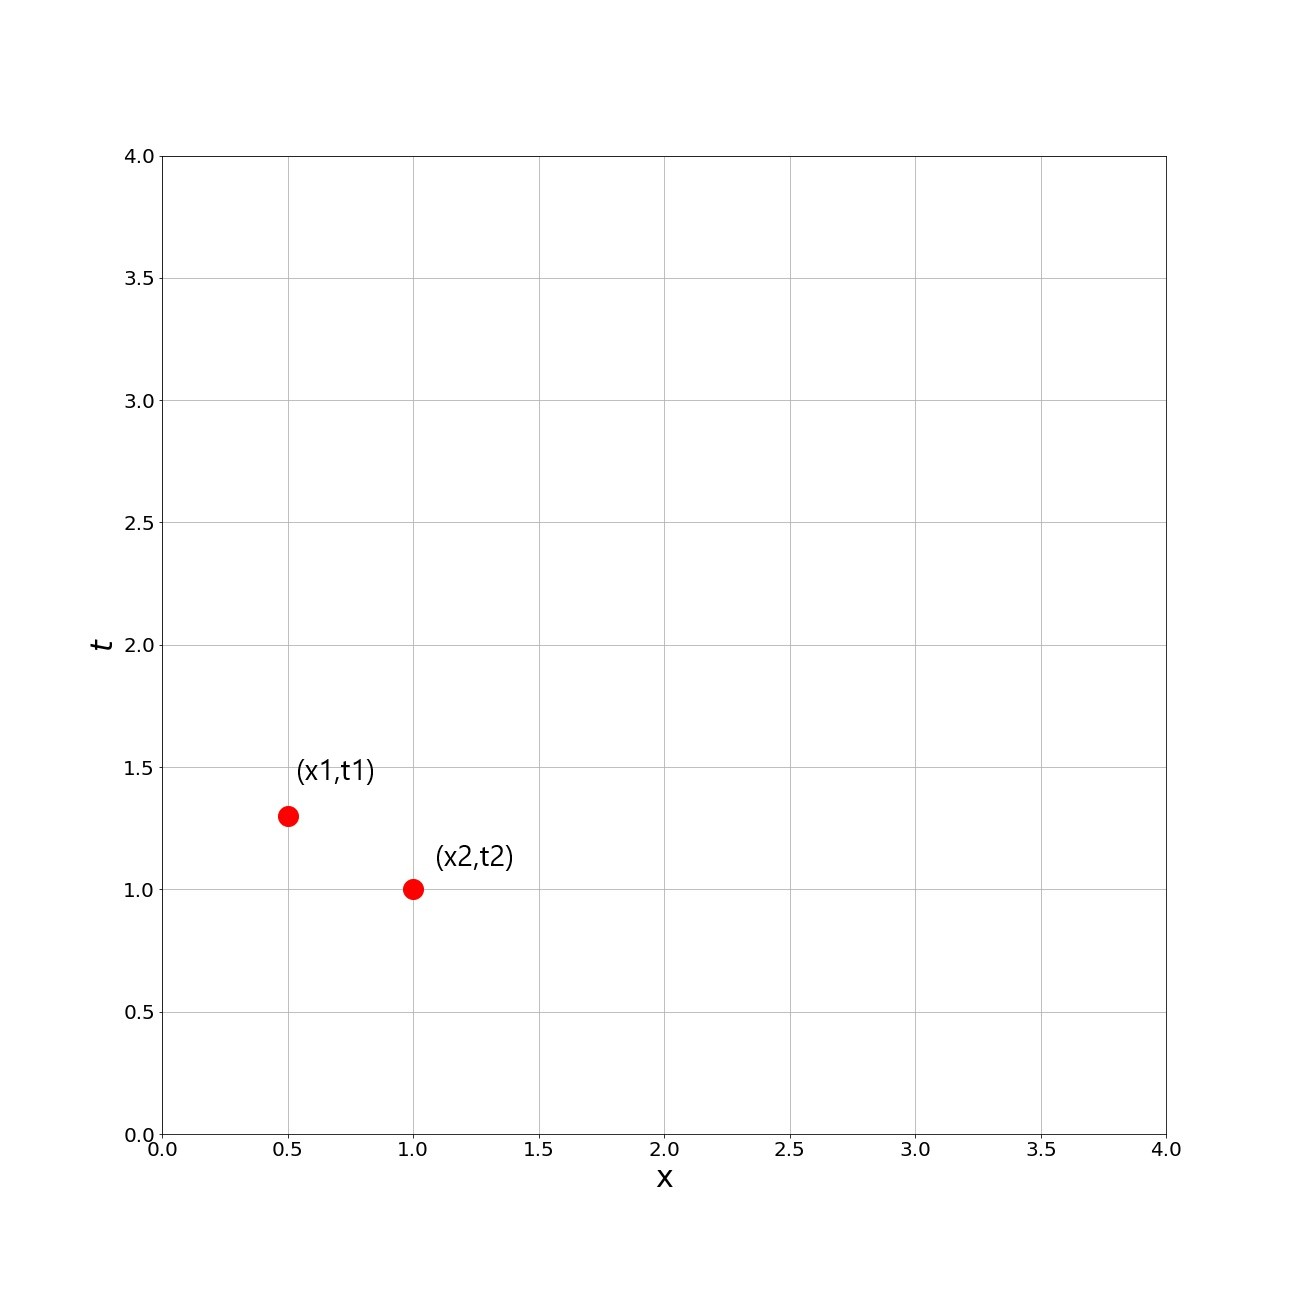
\includegraphics[width=90mm]{img/SampleGaussianProcesses.jpg} \\
    (c) Function estimated from the multivariate Gaussian. Correspond to the white dot in (b)
\end{center}

In practice we can't work in an infinite space. In fact, we operate over the finite set of the training data. This process will produce a distribution which describe t. This distribution can be used to make prediction for never seen inputs.
Now we will explain how we can define a prior distribution over the functions. To do so we recall what we did for linear Bayesian regression. So taken a generic parametric model we have
\begin{equation*}
    y(x,w)=w^T \Phi(x)
\end{equation*}
In the case of ridge regression we have that the prior over w is
\begin{equation*}
    w \sim \mathcal{N}(w|0, \tau I)
\end{equation*}
So how is y distributed? We know that the linear combination of Gaussian is still Gaussian. So knowing that y is a linear combination of w, we are sure that it is distributed as a Gaussian. Now we can calculate its mean and variance.
\begin{align*}
    E[y] &= \Phi E[w] = 0 \\
    Cov[y] &= E[yy^T] = \Phi E[ww^T] \Phi^T = \tau \Phi \Phi^T = K, \text{ Gram matrix}\\
    K_{nm} &= k(x_n, x_m) = \tau\Phi(x_n)^T\Phi(x_m)
\end{align*}
So we have
\begin{equation}
    y \sim \mathcal{N}(y|0, K)
\end{equation}
To justify why K is the covariance matrix of y, we can observe that the Gram matrix components are the kernel function values of input pairs. We have said that the kernel function measure the similarity between two inputs. So K measure the similarity between all inputs pairs and so the correlation of the outputs y.
Now we can define a more formal and organized definition of Gaussian processes.
\begin{definition}[Gaussian process]
A Gaussian process is defined as a probability distribution over function y(x), such that the set of values of y(x), evaluated at an arbitrary set of point $\{x_1, \dots, x_N\}$, jointly have a Gaussian distribution
\end{definition}
Being a Gaussian, the distribution can be completely specified by the mean and covariance.
\paragraph{Note - Fitting} As for every kernel method, the choice of the kernel is very important, because it defines how the inputs are correlated. A hyperparameter which control the under-overfitting of the method is the bandwidth of the Gaussian ($\sigma$). A narrow bandwidth means that inputs near each other will be highly correlated and the correlation between inputs will decrease very fast as we increase the "distance" between the inputs. On the other hand, for wider bandwidth even slightly far away inputs will be correlated. In case of overfitting we would like to use wider bandwidth because the sample will be less correlated locally, thus decreasing the probability of fitting the noise. From another point of view, if we increase the bandwidth every inputs will "see" more inputs ,and so it will have more samples to estimate the function value. In the same way, if we are underfitting we can have narrower bandwidth.

\subsubsection{Prediction}
In this section we will see how we can predict the value of our function in input points never seen before. We consider the case in which we use Gaussian processes for regression. As usual for every regression method we define our target value as
\begin{equation*}
    t_n = y(x_n) + \epsilon,\text{ where } \ \epsilon \sim \mathcal{N}(0, \sigma^2)
\end{equation*}
Under the assumption that the noise is distributed as a Gaussian, we can say that the conditional distribution
\begin{equation}
    P(t_n|y_n) = \mathcal{N}(t_n|y_n(x_n), \sigma^2)
\end{equation}
We can also assume that the noise is independent on each data point. So the joint distribution of t is still Gaussian
\begin{equation}
    p(t|y) = \mathcal{N}(t|y, \sigma^2 I)
\end{equation}
Since $p(y)=\mathcal{N}(0, K)$, we can compute the marginal distribution $p(t)$\footnotemark \footnotetext{As $p(w)$ is the prior in liner Bayesian regression, $p(t)$ is the prior with Gaussian processes}
\begin{equation}
    p(t) = \int p(t|y)p(y)dy = \mathcal{N}(t|0,C),\text{where } C = K + \sigma^2 I_N
\end{equation}
Now suppose we want to make a prediction $t_{N+1}$ for a new data input $x_{N+1}$, given the training data. Our goal is to evaluate the predictive distribution $p(t_{N+1}|t^{(N)},x_1,\dots,x_N+1)$\footnotemark \footnotetext{$t^{(N)}$ is the $t$ vector when we have N sample. The professor in the lecture uses $\pmb{t}_N$ but I found it a little misleading, because the difference between the bold character and the normal one can be easily missed. Also putting the number of sample as a superscript reminds of the iterations count in other notation}
We can calculate that
\begin{align*}
    p(t^{(N+1)}) &= \mathcal{N}(t^{(N+1)}|0,C^{(N+1)}), \text{ where} \\
    C^{(N+1)} &= 
    \begin{bmatrix} 
    C^{(N)} & k \\
    k^T & c
    \end{bmatrix}, \quad [(N+1) x (N+1)] \\
    k &= \begin{bmatrix} k(x_1, x_{N+1}) & \dots & k(x_N, x_{N+1}) \end{bmatrix}^T, \quad [Nx1] \\
    c &= k(x_{N+1},x_{N+1}), \quad [1x1]
\end{align*}
We can observe that for the Gaussian distribution properties, the predictive distribution is still a Gaussian. From that, we can apply the properties over conditional Gaussian distribution to obtain $p(t_{N+1}|t^{(N)},x_1,\dots,x_N+1)$.
\begin{equation}
    p(t_{N+1}|t^{(N)},x_1,\dots,x_N+1) \sim \mathcal{N}(t_{N+1}|k^T {C^{(N)}}^{-1} t, c - k^T {C^{(N)}}^{-1} k)
\end{equation}
We can observe two things. The mean and the variance depend on $x_{N+1}$. More interestingly, the mean of the prediction is actually what we obtain for the kernel version of ridge regression. This shouldn't be a surprise, because we have already said that in the parametric word, ridge regression is a particular case of linear Bayesian regression, when the prior is Gaussian and centered around zero. So this particular case holds also in the kernel world.
We see that to calculate our prediction we need to invert C. This operation is always possible because by definition K is a Gram matrix and so its semi-definite positive. If we add to K $\sigma^2 I$, we are sure that C is positive definite and so it is for sure invertible.
\paragraph{Note - computational cost} As usual, inverting a matrix is the most intensive operation of the solution. In our case, the complexity of inverting C will be $\mathcal{O}(N^3)$. Luckily we need to compute this only one once for the given training set. We can also observe that the complexity depends only on the number of samples, as it should be for kernel methods. When we obtain a new sample, we can use the already calculated ${C^{(N)}}^{-1}$ to simplify the complexity of calculating the mean and variance of the predictive distribution. Indeed, we have that the computational cost of the mean is $\mathcal{O}(N)$ and of the variance is $\mathcal{O}(N^2)$. For large dataset is very expensive to calculate exactly the result, so we resort to approximated methods like random sampling and clustering.

\paragraph{Example - Prediction} Suppose to have a regression problem we want to solve with Gaussian processes. For simplicity we assume that our function is described by $t_1$ and $t_2$, which are the function value for $x_1$ and $x_2$. 
First, we construct our prior p(t) (red ellipses). We assume a zero mean distribution, where the shape of the multivariate Gaussian prior depends on the covariance matrix, and so on the kernel we choose. Now we haven't observed any data, so our best guess for both $t_1$ and $t_2$ is zero. Now we observe in $x_1$ a value for $t_1$(blue dot). We know that $t_1$ and $t_2$ are correlated, so observing $t_1$ will give us some information about $t_2$. We know that the predictive distribution $p(t_2|t_1, x_1, x_2)$(green Gaussian) is a Gaussian. In the prior plot below we can visualize this distribution through cutting the prior $p(t)$ parallel to $t_2$ through $t_1$(blue line). This slice of $p(t)$ will be $p(t_2|t_1, x_1, x_2)$. Now we can take the mean to estimate $t_2$(green point).

As we have said before, like we need to define features in the parametric world, we need to define a kernel in the non-parametric case. In some cases, the kernel have some hyperparameters. How can we find the optimal values for this hyperparameters?
We have already seen how cross validation can be used to do model selection. This method is very robust, but at the same time it is slow. Another approach uses the maximization of the marginal likelihood using gradient optimization. In practice, you want to find the hyperparameters for which the observed target variables are more likely. This is faster, but it can be stuck in local minima. Usually the gradient approach is the go to method for hyperparameters optimization.
\end{document}
